%\begin{slide}{６．４　部分積分(integration by parts)　}
%\begin{itemize}
%\item 関数$f(x),g(x)$の掛け算の微分は$(f(x)g(x))'=f'(x)g(x) + f(x)g'(x)$なので、両辺を積分すると
%\begin{equation}
%f(x)g(x) = \int f'(x)g(x) dx + \int f(x)g'(x) dx \nonumber
%\end{equation}
%したがって
%\begin{equation}
%\int f'(x)g(x) dx = f(x)g(x) - \int f(x)g'(x) dx \label{eq:ibyp}
%\end{equation}
%式(\ref{eq:ibyp})を部分積分の公式という。\red{微分して簡単化できる関数を$g(x)$に選ぶことがポイント。}
%\end{itemize}
%\end{slide}
%\begin{slide}{例題6.4}
%積分せよ
%\begin{itemize}
%\item $\int x\cos{x}dx$
%
%解答例: $g(x)=x$, $f'(x)=\cos{x}$とすると
%\begin{equation}
%g'(x) = 1,  \qquad f(x) = \sin{x} \nonumber 
%\end{equation}
%なので部分積分を用いて
%\begin{equation}
%\int x\cos{x}dx = x\sin{x} - \int \sin{x} dx =  x\sin{x} + \cos{x} + C \nonumber 
%\end{equation}
%\item $\int e^x(2x+1)dx$
%
%解答例：$f'(x)=e^x$, $g(x)=2x+1$とすると
%\begin{equation}
%f(x) = e^x, \qquad  g'(x) = 2 \nonumber
%\end{equation}
%部分積分を用いて
%\begin{eqnarray}
%&\int& e^x(2x+1)dx = e^x(2x+1) - 2\int e^xdx \nonumber \\
%&=& e^x(2x+1) - 2e^x + C =  e^x(2x-1)+C \nonumber 
%\end{eqnarray}
%\end{itemize}
%\end{slide}
%\begin{slide}{例題6.5}
%積分せよ
%\begin{itemize}
%\item $\int \log_e{x} dx, \qquad x > 0$ 
%
%解説$(\log_e{x})'=\frac{1}{x}$なので、
%\begin{equation}
%g(x) = \log_e{x}, \qquad f'(x) = 1 \nonumber
%\end{equation}
%と考えて
%\begin{eqnarray}
%g'(x) &=& \frac{1}{x} \nonumber \\
%f(x) &=& x \nonumber
%\end{eqnarray}
%なので
%\begin{equation}
%\int \log_e{x} dx = x\log_e{x} + C - \int \frac{1}{x} x dx = x\log_e{x} -x +  C \nonumber 
%\end{equation}
%\end{itemize}
%\end{slide}
%\begin{slide}{部分積分に関する補足}
%\begin{itemize}
%\item $\int \log_e{x} dx$ を積分する際
%
%$(\log_e{x})'=\frac{1}{x}$なので、
%\begin{equation}
%g(x) = \log_e{x}, \qquad f'(x) = 1 \nonumber
%\end{equation}
%とすると不定積分は
%\begin{eqnarray}
%g'(x) &=& \frac{1}{x} \nonumber \\
%f(x) &=& x + C_1\nonumber
%\end{eqnarray}
%となるが、$f(x)$の積分定数はキャンセルされる。
%\begin{eqnarray}
%&\int& \log_e{x} dx = x\log_e{x} + C_1\log_e{x} - \int \frac{1}{x} (x+C_1) dx \nonumber \\
%&=& x\log{x} \cancel{+ C_1\log_e{x}} -x \cancel{- C_1\log_e{x}}+  C \nonumber \\
%&=& x\log{x}  -x +  C \nonumber
%\end{eqnarray}
%\red{部分積分で$f(x)$を求める際に積分定数は省略して問題ない。}
%\end{itemize}
%\end{slide}
%\begin{slide}{例題}
%積分せよ
%\begin{itemize}
%\item $\int \log_e{(x+1)} dx, \qquad (x+1) > 0$
%\item 解答例
%$f'(x)=1, g(x)=\log_e{(x+1)}$とすると$f(x)=x, g'(x)={\frac{1}{x+1}}$となる。部分積分を適用して
%\begin{equation}
%\int \log_e{(x+1)} dx = x\log_e{(x+1)} - \int \frac{x}{x+1} dx \label{eq:pinto} 
%\end{equation}
%$u=x+1$と置換して$\frac{dx}{du} = 1$なので
%\begin{equation}
%\int \frac{x}{x+1} dx = \int \frac{u-1}{u} \frac{dx}{du} du = \int 1-\frac{1}{u} du =  u - \log_e{u} \label{eq:pint}
%\end{equation}
%式\pref{eq:pint}を式\pref{eq:pinto}に代入して
%\begin{eqnarray}
%&& \int \log_e{(x+1)} dx =  x\log_e{(x+1)} - u + \log_e{u}  +C \nonumber \\
%&=& x\log_e{(x+1)} - (x+1) + \log_e{(x+1)} \nonumber \\
%&=& (x+1)\log_e{(x+1)} -x + C\nonumber 
%\end{eqnarray}
%\end{itemize}
%\end{slide}
%\begin{slide}{問題6.4}
%積分せよ
%\begin{itemize}
%\item
%\begin{equation}
%\int x \sin{x} dx \nonumber 
%\end{equation}
%\item 
%\begin{equation}
%\int xe^{-x+1} dx \nonumber 
%\end{equation}
%\item 
%\begin{equation}
%\int \sqrt{x}\log{x} dx \nonumber 
%\end{equation}
%\end{itemize}
%\end{slide}
\begin{frame}
\frametitle{区分求積法}

一般に
\begin{align*}
S_n &= \sum_{k=1}^n  \frac{1}{n} \big(\frac{k}{n}\big)^2 = \frac{1}{n^3}  \sum_{k=1}^n k^2 \\
& =  \frac{1}{n^3} \cdot  \frac{1}{6}n(n+1)(2n+1) = \frac{1}{6} (1+\frac{1}{n})(2+\frac{1}{n})
\end{align*}
より$\displaystyle \lim_{n\to \infty}S_n=\frac{1}{3}$. \\
\ \\

一方で, $S_n-s_n=\frac{1}{n}$に注意すると, $\displaystyle \lim_{n\to \infty}s_n=\frac{1}{3}$なので, 
領域の面積は
$$
S= \lim_{n\to \infty}s_n=\lim_{n\to \infty}S_n=\frac{1}{3}.
$$ 

\end{frame}


%%%%%%%%%%%%%%%%%%%%%%%%%%%%%%%%%%%%%%%%%%%%%%%%%%%%%%%%%%%%%%%%%%%%%%%%%%%%%%%%%%%%%%%
%%%%%%%%%%%%%%%%%%%%%%%%%%%%%%%%%%%%%%%%%%%%%%%%%%%%%%%%%%%%%%%%%%%%%%%%%%%%%%%%%%%%%%

%
%\begin{frame}
%\frametitle{区分求積法 (補足)}
%
%公式$\displaystyle \sum_{k=1}^n k^2=  \frac{1}{6}n(n+1)(2n+1)$を示す. 恒等式
%$$
%(k+1)^3-k^3=3k^2+3k+1
%$$
%の両辺を$k=1$から$n$まで和を取ることを考える. 
%\begin{align*}
%\text{左辺の和} & = (n+1)^3-n^3+n^3-(n-1)^3+\dots3^3-2^3+2^3-1^3\\
%& = (n+1)^3-1=n^3+3n^2+3n. \\
%\text{右辺の和} &= 3\sum_{k=1}^n k^2+3\sum_{k=1}^n k+\sum_{k=1}^n 1=  3\sum_{k=1}^n k^2+3\frac{n(n+1)}{2}+n. 
%\end{align*}
%両辺を整理すると
%$$
%\sum_{k=1}^n k^2 = \frac{1}{3}(n^3+3n^2+3n-3\frac{n(n+1)}{2}-n)
%=  \frac{1}{6}n(n+1)(2n+1). 
%$$
%
%\end{frame}


%%%%%%%%%%%%%%%%%%%%%%%%%%%%%%%%%%%%%%%%%%%%%%%%%%%%%%%%%%%%%%%%%%%%%%%%%%%%%%%%%%%%%%%
%%%%%%%%%%%%%%%%%%%%%%%%%%%%%%%%%%%%%%%%%%%%%%%%%%%%%%%%%%%%%%%%%%%%%%%%%%%%%%%%%%%%%%


\begin{frame}
\frametitle{区分求積法}

一般の関数$f(x)$について考える. 
まずは$f(x) \ge 0$のとき, $f(x)$のグラフ, $x$-軸, 直線$x=a$, $x=b$で囲まれた領域を考える. 
区間$[a,b]$を$n$等分する小区間の幅を$\Delta x = (b-a)/n$とおく. 

\vspace{-2mm}

\begin{figure}[htbp]
 \begin{center} 
  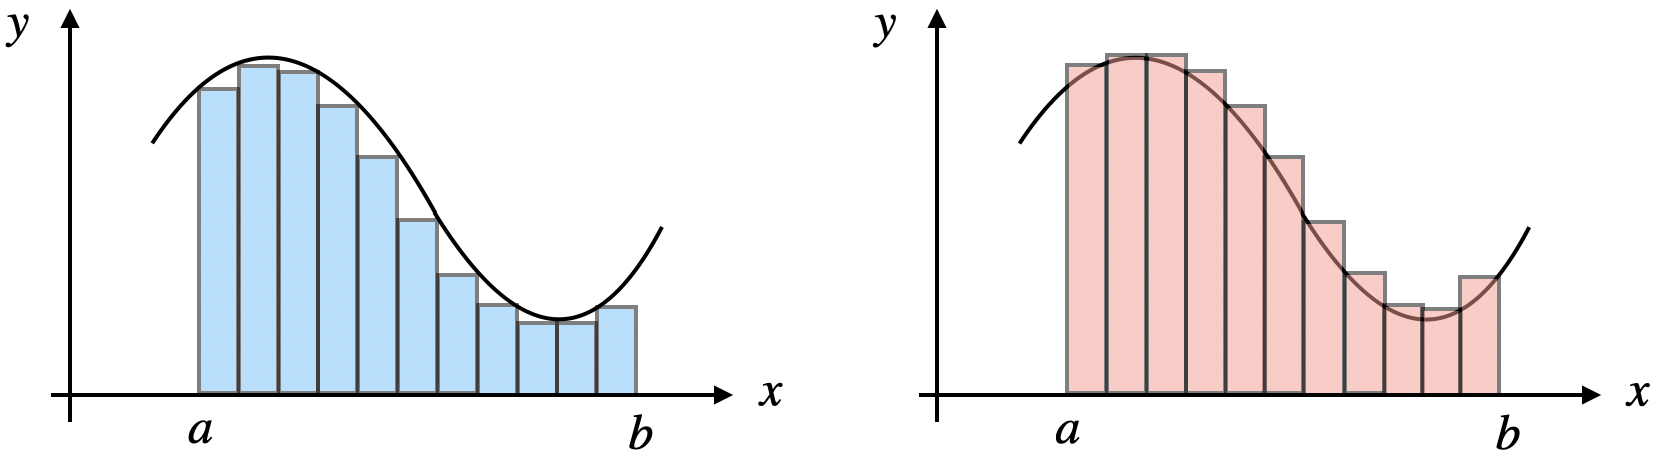
\includegraphics[width=90mm]{calculus12/RiemannSum3.png}
 \end{center}
\end{figure}

\vspace{-2mm}


$k$番目の小区間において, $f(x)$の最小値を与える点を$x_k$, 最大値を与える点を$X_k$とし, 
領域を内側と外側から近似する長方形の集まりの面積をそれぞれ$s_n$, $S_n$とすると
$$
s_n=\sum_{k=1}^nf(x_k)\Delta x, \ \ \ S_n=\sum_{k=1}^nf(X_k)\Delta x
$$




\end{frame}
\begin{slide}{問題６．５}
次の極限を求めよ
\begin{itemize}
\item 
\begin{equation}
A = \lim_{n\to \infty} \left(\frac{1^2}{n^3}+\frac{2^2}{n^3}+\cdots+\frac{n^2}{n^3}\right) \nonumber
\end{equation}
\item 
\begin{equation}
A = \lim_{n\to \infty}\frac{1}{n\sqrt{n}}\left(\sqrt{1}+\sqrt{2}+\cdots+\sqrt{n}\right) \nonumber
\end{equation}
\end{itemize}
\end{slide}

\begin{slide}{例題 6.6}
以下の極限を求めよ
\begin{equation}
A=\lim_{n\to \infty}\left(\frac{1^3}{n^4} + \frac{2^3}{n^4} +\cdots + \frac{n^3}{n^4}\right) \nonumber
\end{equation}

解答例：式を変形すると
\begin{equation}
A = \lim_{n\to \infty} \left(\frac{1^3}{n^3} + \frac{2^3}{n^3} + \cdots + \frac{n^3}{n^3}\right)\frac{1}{n} \nonumber
\end{equation}
となるため、$0 \leqq x \leqq 1$の範囲の$f(x)=x^3$と積分と等価である。したがって
\begin{equation}
\int_0^1 x^3 dx = \left[\frac{1}{4}x^4 \right]_0^1 = \frac{1}{4} \nonumber
\end{equation}
\end{slide}
%%%%%%%%%%%%%%%%%%%%%%%%%%%%%%%%%%%%%%%%%%%%%%%%%%%%%%%%%%%%%%%%%%%%%%%%%%%%%%%%%%%%%%%
%%%%%%%%%%%%%%%%%%%%%%%%%%%%%%%%%%%%%%%%%%%%%%%%%%%%%%%%%%%%%%%%%%%%%%%%%%%%%%%%%%%%%%


\begin{frame}
\frametitle{リーマン和}

\begin{itemize}
\item $s_n=\sum_{k=1}^nf(x_k)\Delta x$は\underline{下ダルブー和}と呼ばれ, $s_1 \le s_2 \le \dots$. 
$$S_*=\lim_{n \to \infty} s_n$$
を区間$[a,b]$における$f(x)$の\underline{下積分}という. 
\item $S_n=\sum_{k=1}^nf(X_k)\Delta x$は\underline{上ダルブー和}と呼ばれ, $S_1 \ge S_2 \ge \dots$. 
$$S^*=\lim_{n \to \infty} S_n$$
を区間$[a,b]$における$f(x)$の\underline{上積分}という. 
\end{itemize}
(有界な単調増加(減少)数列であることから収束が保証される.)

\end{frame}



%%%%%%%%%%%%%%%%%%%%%%%%%%%%%%%%%%%%%%%%%%%%%%%%%%%%%%%%%%%%%%%%%%%%%%%%%%%%%%%%%%%%%%%
%%%%%%%%%%%%%%%%%%%%%%%%%%%%%%%%%%%%%%%%%%%%%%%%%%%%%%%%%%%%%%%%%%%%%%%%%%%%%%%%%%%%%%


\begin{frame}
\frametitle{リーマン積分}


\begin{Def}
下積分$S_*$と上積分$S^*$が一致するとき, $f(x)$は\underline{リーマン積分可能}といい, その値$S_*=S^*$を
$$
\int_a^b f(x)dx
$$
と表す. この値を$f(x)$の\underline{リーマン積分}, もしくは\underline{定積分}という. 
$f(x)$は被積分関数, $[a,b]$は積分区間, $a$は下端, $b$は上端と呼ばれる. 
\end{Def}

一般に, $\sum_{k=1}^nf(x_k^*)\Delta x$の形の和をリーマン和という($x_k^*$は$k$番目の小区間の点). 
$n \to \infty$のとき, リーマン和が$x_k^*$の取り方に依らずある値に収束することとリーマン積分可能性は同値であり, 
その極限値がリーマン積分である.  

\end{frame}


%%%%%%%%%%%%%%%%%%%%%%%%%%%%%%%%%%%%%%%%%%%%%%%%%%%%%%%%%%%%%%%%%%%%%%%%%%%%%%%%%%%%%%%
%%%%%%%%%%%%%%%%%%%%%%%%%%%%%%%%%%%%%%%%%%%%%%%%%%%%%%%%%%%%%%%%%%%%%%%%%%%%%%%%%%%%%%


\begin{frame}
\frametitle{リーマン積分不可能な関数}

不連続関数
$$
f(x)=
\begin{cases}
1 & (x \in \Q)\\
0 & (x \notin \Q)
\end{cases}
$$
を考える. 
任意の小区間において有理数と無理数はどちらも存在するため
\begin{align*}
s_n &= \sum_{k=1}^nf(x_k)\Delta x = \sum_{k=1}^n 0 \cdot \Delta x =0, \\
S_n &= \sum_{k=1}^nf(X_k)\Delta x = \sum_{k=1}^n 1 \cdot \Delta x =n \Delta x = b-a. 
\end{align*}
上積分と下積分が一致しないので, $f(x)$はリーマン積分不可能. \\
\ \\

一方で, 連続な関数はリーマン積分可能であることが知られている. 
\end{frame}



%%%%%%%%%%%%%%%%%%%%%%%%%%%%%%%%%%%%%%%%%%%%%%%%%%%%%%%%%%%%%%%%%%%%%%%%%%%%%%%%%%%%%%%
%%%%%%%%%%%%%%%%%%%%%%%%%%%%%%%%%%%%%%%%%%%%%%%%%%%%%%%%%%%%%%%%%%%%%%%%%%%%%%%%%%%%%%


\begin{frame}
\frametitle{リーマン積分}

\vspace{-3mm}

\begin{figure}[htbp]
 \begin{center} 
  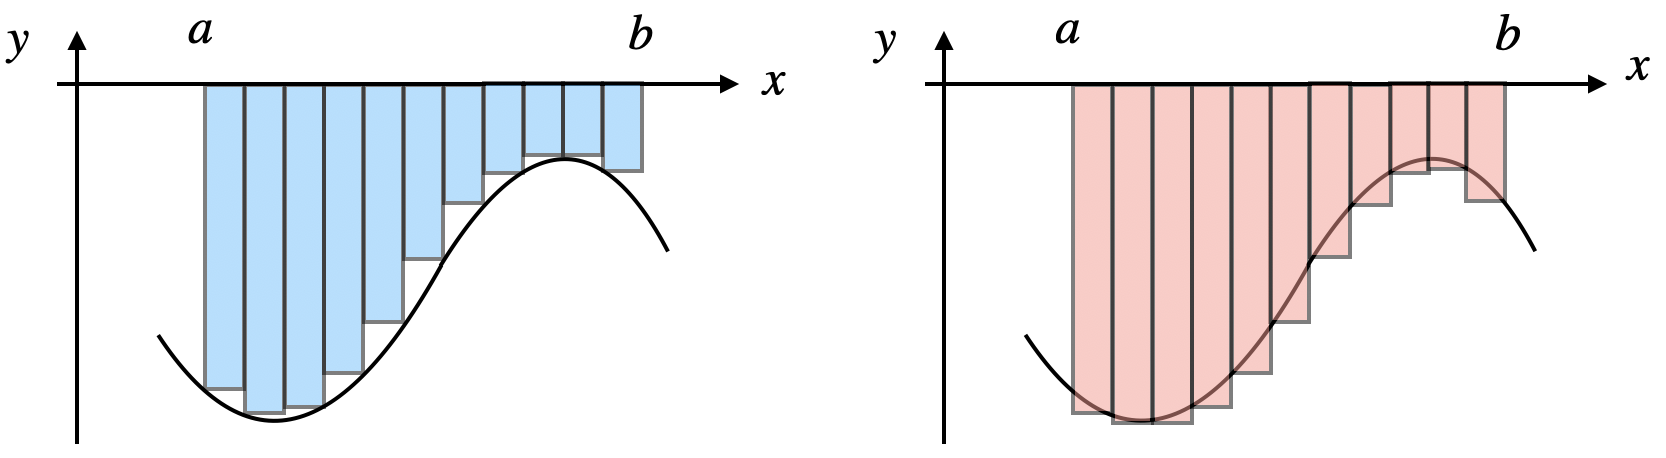
\includegraphics[width=90mm]{calculus12/RiemannSum4.png}
 \end{center}
\end{figure}

\vspace{-3mm}

これまで被積分関数が積分区間上で非負の場合を考えたが, 一般の場合でも定積分は考えられる. 
まず$f(x) \le 0$の場合も同様に積分区間を分割して, 上下のダルブー和を計算する
$$
s_n = \sum_{k=1}^nf(x_k)\Delta x, \ \ \ S_n = \sum_{k=1}^nf(X_k)\Delta x
$$
$x_k$は$k$番目の小区間での$f(x)$の最大値を与える点, $X_k$は最小値を与える点である. 
$\displaystyle \lim_{n\to \infty} s_n = \lim_{n\to \infty} S_n$であるとき, その値を定積分
$\int_a^b f(x)dx$と定める. 


\end{frame}



%%%%%%%%%%%%%%%%%%%%%%%%%%%%%%%%%%%%%%%%%%%%%%%%%%%%%%%%%%%%%%%%%%%%%%%%%%%%%%%%%%%%%%%
%%%%%%%%%%%%%%%%%%%%%%%%%%%%%%%%%%%%%%%%%%%%%%%%%%%%%%%%%%%%%%%%%%%%%%%%%%%%%%%%%%%%%%


\begin{frame}
\frametitle{リーマン積分}


$f(x) \le 0$のとき, $f(x)$の定積分$\int_a^b f(x)dx$は, $f(x)$のグラフ, $x$-軸, 直線$x=a$, $x=b$で囲まれた領域の面積の逆符号を与える. \\
\ \\

一般の関数$f(x)$の定積分は, $f(x)$のグラフ, $x$-軸, 直線$x=a$, $x=b$で囲まれた領域のうち, 
$x$-軸より上の部分の面積を正, 下の部分の面積を負として足し合わせた値として定める. 

\vspace{-1mm}

\begin{figure}[htbp]
 \begin{center} 
  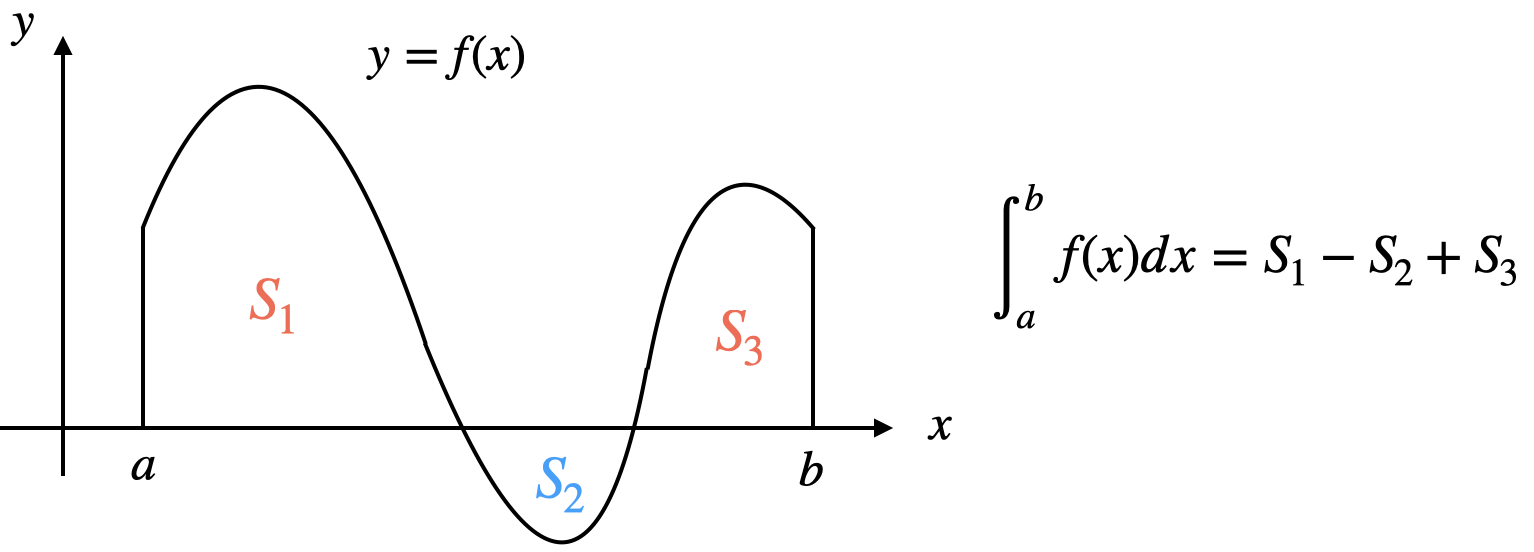
\includegraphics[width=100mm]{calculus12/RiemannInt.png}
 \end{center}
\end{figure}

\vspace{-1mm}

\end{frame}


%%%%%%%%%%%%%%%%%%%%%%%%%%%%%%%%%%%%%%%%%%%%%%%%%%%%%%%%%%%%%%%%%%%%%%%%%%%%%%%%%%%%%%%
%%%%%%%%%%%%%%%%%%%%%%%%%%%%%%%%%%%%%%%%%%%%%%%%%%%%%%%%%%%%%%%%%%%%%%%%%%%%%%%%%%%%%%


\begin{frame}
\frametitle{定積分の性質}

$a,b$の大小が異なる場合も扱えるように, $\int_b^a f(x)dx =- \int_a^b f(x)dx$と定義する. 
定積分は次の性質を持つ. 

\begin{itemize}
\item $\displaystyle \int_a^b (k f(x)+l g(x))dx =  k \int_a^b f(x)dx + l \int_a^b g(x)dx$
\item $\displaystyle f(x) \le g(x) \Longrightarrow  \int_a^b f(x)dx \le \int_a^b g(x)dx$
\item $\displaystyle \big| \int_a^b f(x)dx \big| \le \int_a^b |f(x)|dx \ \ \ (a \le b)$
\item $\displaystyle  \int_a^c f(x)dx = \int_a^b f(x)dx + \int_b^c f(x)dx$
\end{itemize}
ただし$k,l \in \R$. 

\end{frame}


%%%%%%%%%%%%%%%%%%%%%%%%%%%%%%%%%%%%%%%%%%%%%%%%%%%%%%%%%%%%%%%%%%%%%%%%%%%%%%%%%%%%%%%
%%%%%%%%%%%%%%%%%%%%%%%%%%%%%%%%%%%%%%%%%%%%%%%%%%%%%%%%%%%%%%%%%%%%%%%%%%%%%%%%%%%%%%


\begin{frame}
\frametitle{積分の平均値の定理}


\begin{Thm}[積分の平均値の定理]
連続関数$f(x)$に関して
$$
\int_a^b f(x)dx = f(c)(b-a)
$$
を満たす$c \in (a,b)$が存在する. 
\end{Thm}
%証明は連続関数に関する中間値の定理による. 

\begin{figure}[htbp]
 \begin{center} 
  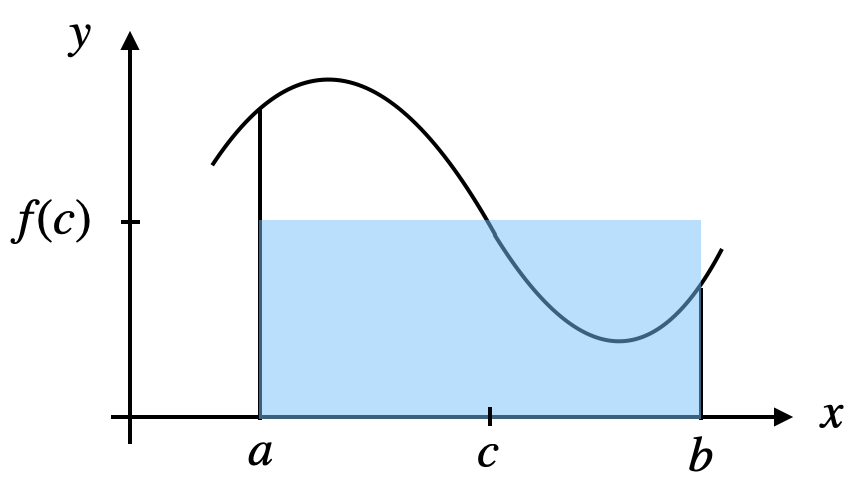
\includegraphics[width=55mm]{calculus12/MeanValueInt.png}
 \end{center}
\end{figure}

\end{frame}


%%%%%%%%%%%%%%%%%%%%%%%%%%%%%%%%%%%%%%%%%%%%%%%%%%%%%%%%%%%%%%%%%%%%%%%%%%%%%%%%%%%%%%%
%%%%%%%%%%%%%%%%%%%%%%%%%%%%%%%%%%%%%%%%%%%%%%%%%%%%%%%%%%%%%%%%%%%%%%%%%%%%%%%%%%%%%%


\begin{frame}
\frametitle{積分の平均値の定理の証明}

ワイエルシュトラスの定理より, 連続関数$f(x)$は$[a,b]$において最大値$M$と最小値$m$を持ち, 
$$
m(b-a) \le \int_a^b f(x)dx \le M(b-a). 
$$
これより
$$
m \le \frac{1}{b-a}\int_a^b f(x)dx \le M.  
$$
連続関数に関する中間値の定理より
$$
\frac{1}{b-a}\int_a^b f(x)dx = f(c)
$$
を満たす$c \in (a,b)$が存在する. 


\end{frame}



%%%%%%%%%%%%%%%%%%%%%%%%%%%%%%%%%%%%%%%%%%%%%%%%%%%%%%%%%%%%%%%%%%%%%%%%%%%%%%%%%%%%%%%
%%%%%%%%%%%%%%%%%%%%%%%%%%%%%%%%%%%%%%%%%%%%%%%%%%%%%%%%%%%%%%%%%%%%%%%%%%%%%%%%%%%%%%%

%%%%%%%%%%%%%%%%%%%%%%%%%%%%%%%%%%%%%%%%%%%%%%%%%%%%%%%%%%%%%%%%%%%%%%%%%%%%%%%%%%%%%%%
%%%%%%%%%%%%%%%%%%%%%%%%%%%%%%%%%%%%%%%%%%%%%%%%%%%%%%%%%%%%%%%%%%%%%%%%%%%%%%%%%%%%%%

\section{定積分と不定積分}

\begin{frame}
\frametitle{微積分学の基本定理}


\begin{Thm}[微積分学の基本定理]
連続関数$f(x)$に対して, 定積分で定まる関数
$$
S(x)=\int_a^x f(t)dt
$$
は$f(x)$の原始関数, つまり
$$
S'(x)= \frac{d}{dx} \int_a^x f(t)dt = f(x).
$$
\end{Thm}
特に
$$
S(c)-S(b)= \int_a^c f(t)dt-\int_a^b f(t)dt = \int_b^c f(t)dt. 
$$

\end{frame}


%%%%%%%%%%%%%%%%%%%%%%%%%%%%%%%%%%%%%%%%%%%%%%%%%%%%%%%%%%%%%%%%%%%%%%%%%%%%%%%%%%%%%%%
%%%%%%%%%%%%%%%%%%%%%%%%%%%%%%%%%%%%%%%%%%%%%%%%%%%%%%%%%%%%%%%%%%%%%%%%%%%%%%%%%%%%%%

\begin{frame}
\frametitle{微積分学の基本定理の証明}


$$
S(x+h)-S(x)=\int_a^{x+h} f(t)dt - \int_a^{x} f(t)dt = \int_x^{x+h} f(t)dt
$$
であるが, 積分の平均値の定理より
$$
\int_x^{x+h} f(t)dt = f(c)h
$$
なる$c \in (x,x+h)$が存在する. 
$h \to 0$とすると, $c \to x$であるので
$$
S'(x)=\lim_{h \to 0} \frac{S(x+h)-S(x)}{h}=\lim_{h \to 0}\frac{f(c)h}{h}=f(x).
$$
(厳密には$h$の正負で場合分けが必要.)

\end{frame}


%%%%%%%%%%%%%%%%%%%%%%%%%%%%%%%%%%%%%%%%%%%%%%%%%%%%%%%%%%%%%%%%%%%%%%%%%%%%%%%%%%%%%%%
%%%%%%%%%%%%%%%%%%%%%%%%%%%%%%%%%%%%%%%%%%%%%%%%%%%%%%%%%%%%%%%%%%%%%%%%%%%%%%%%%%%%%%

\begin{frame}
\frametitle{定積分と不定積分の関係}

\begin{Thm}
$f(x)$の原始関数の一つを$F(x)$とするとき
$$
\int_a^b f(x)dx=F(b)-F(a)=:\big[F(x)\big]_a^b
$$
つまり, 定積分は区分求積法を用いなくとも原始関数から計算可能.  
\end{Thm}
原始関数$F(x)$は無数に存在するが, 先ほど定義した$S(x)$と定数$C$を用いて$F(x)=S(x)+C$と書けるので
$$
F(b)-F(a)=(S(b)+C)-(S(a)+C)=\int_a^bf(x)dx. 
$$

\end{frame}


%%%%%%%%%%%%%%%%%%%%%%%%%%%%%%%%%%%%%%%%%%%%%%%%%%%%%%%%%%%%%%%%%%%%%%%%%%%%%%%%%%%%%%%
%%%%%%%%%%%%%%%%%%%%%%%%%%%%%%%%%%%%%%%%%%%%%%%%%%%%%%%%%%%%%%%%%%%%%%%%%%%%%%%%%%%%%%

\section{定積分の計算}

\begin{frame}
\frametitle{定積分の計算例}

\begin{align*}
\int_1^2(3x^2+4x-1)dx & = \big[x^3+2x^2-x\big]_1^2 \\
& = (2^3+2\cdot 2^2-2)-(1^3+2\cdot 1^2-1) \\
& = 12. 
\end{align*}


\begin{align*}
\int_0^\pi \sin x dx & = \big[ -\cos x\big]_0^\pi \\
& = -\cos \pi - (- \cos 0) \\
& = 2. 
\end{align*}

\end{frame}


%%%%%%%%%%%%%%%%%%%%%%%%%%%%%%%%%%%%%%%%%%%%%%%%%%%%%%%%%%%%%%%%%%%%%%%%%%%%%%%%%%%%%%%
%%%%%%%%%%%%%%%%%%%%%%%%%%%%%%%%%%%%%%%%%%%%%%%%%%%%%%%%%%%%%%%%%%%%%%%%%%%%%%%%%%%%%%


\begin{frame}
\frametitle{定積分の計算例}

\begin{align*}
\int_1^e\frac{1+x^2}{x}dx & = \int_1^e(\frac{1}{x}+x)dx \\
& = \big[ \log x + \frac{1}{2}x^2\big]_1^e \\
& = (\log e + \frac{e^2}{2})-(\log 1 +\frac{1}{2})\\
& = \frac{e^2+1}{2}. 
\end{align*}


\end{frame}


%%%%%%%%%%%%%%%%%%%%%%%%%%%%%%%%%%%%%%%%%%%%%%%%%%%%%%%%%%%%%%%%%%%%%%%%%%%%%%%%%%%%%%%
%%%%%%%%%%%%%%%%%%%%%%%%%%%%%%%%%%%%%%%%%%%%%%%%%%%%%%%%%%%%%%%%%%%%%%%%%%%%%%%%%%%%%%


\begin{frame}
\frametitle{定積分の計算例}


\begin{align*}
\int_0^{2\pi} \sin x dx & = \big[ -\cos x\big]_0^{2\pi} \\
& = -\cos 2\pi - (- \cos 0) \\
& =0. 
\end{align*}

\begin{align*}
\int_0^{2\pi} |\sin x| dx & = \int_0^{\pi} \sin x dx + \int_\pi^{2\pi} (-\sin x) dx \\
& = \big[ -\cos x\big]_0^{\pi} +  \big[ \cos x\big]_\pi^{2\pi} \\
& = -\cos \pi - (- \cos 0) + \cos 2\pi - \cos \pi \\
& =4. 
\end{align*}

\end{frame}



%%%%%%%%%%%%%%%%%%%%%%%%%%%%%%%%%%%%%%%%%%%%%%%%%%%%%%%%%%%%%%%%%%%%%%%%%%%%%%%%%%%%%%%
%%%%%%%%%%%%%%%%%%%%%%%%%%%%%%%%%%%%%%%%%%%%%%%%%%%%%%%%%%%%%%%%%%%%%%%%%%%%%%%%%%%%%%


\section{部分積分}

\begin{frame}
\frametitle{部分積分}

\vspace{-2.7mm}

\begin{Thm}[部分積分の公式] \vspace{-1mm}
$$
\int_a^b f(x)g'(x)dx = \big[f(x)g(x)\big]_a^b - \int_a^b f'(x)g(x)dx
$$
\end{Thm} \vspace{-0.5mm}
実際, 不定積分の部分積分の公式
$$
\int f(x)g'(x)dx = f(x)g(x) - \int f'(x)g(x)dx
$$
より$H(x)=f(x)g(x) - \int_c^x f'(t)g(t)dt$は$ f(x)g'(x)$の原始関数なので \vspace{-1mm}
\begin{align*}
\int_a^b f(x)g'(x)dx &= H(b)-H(a) \\
& = f(b)g(b) - \int_c^b f'(t)g(t)dt - (f(a)g(a) - \int_c^a f'(t)g(t)dt) \\
& = \big[f(x)g(x)\big]_a^b - \int_a^b f'(x)g(x)dx. 
\end{align*}


\end{frame}

%%%%%%%%%%%%%%%%%%%%%%%%%%%%%%%%%%%%%%%%%%%%%%%%%%%%%%%%%%%%%%%%%%%%%%%%%%%%%%%%%%%%%%%
%%%%%%%%%%%%%%%%%%%%%%%%%%%%%%%%%%%%%%%%%%%%%%%%%%%%%%%%%%%%%%%%%%%%%%%%%%%%%%%%%%%%%%


\begin{frame}
\frametitle{部分積分の計算例}


\begin{align*}
\int_1^{e} 4 x \log x dx & = \big[ 2x^2 \log x \big]_1^{e}- \int_1^e 2x^2 \cdot \frac{1}{x}dx \\
& = 2e^2 \log e - 2 \log 1 - \int_1^e2xdx \\
& = 2e^2-\big[x^2\big]_1^e = e^2+1. 
\end{align*}

\begin{align*}
\int_0^{\frac{\pi}{2}} x \cos x  dx & = \big[ x \sin x \big]_0^{\frac{\pi}{2}} - \int_0^{\frac{\pi}{2}} \sin x dx \\
& = \frac{\pi}{2}-0-\big[-\cos x \big]_0^{\frac{\pi}{2}}= \frac{\pi}{2}-1. 
\end{align*}

\end{frame}


%%%%%%%%%%%%%%%%%%%%%%%%%%%%%%%%%%%%%%%%%%%%%%%%%%%%%%%%%%%%%%%%%%%%%%%%%%%%%%%%%%%%%%%
%%%%%%%%%%%%%%%%%%%%%%%%%%%%%%%%%%%%%%%%%%%%%%%%%%%%%%%%%%%%%%%%%%%%%%%%%%%%%%%%%%%%%%

\section{置換積分}

\begin{frame}
\frametitle{置換積分}

\begin{Thm}[置換積分の公式] 
関数$f(x)$の変数$x$が別の変数$t$の$C^1$級関数$x=\phi(t)$として表されるとき
$$
\int_a^b f(x)dx =\int_\alpha^\beta f(\phi(t))\phi'(t)dt
$$
ただし, $\phi(\alpha)=a$,  $\phi(\beta)=b$である. 
\end{Thm}
実際, 不定積分の置換公式
$$
\int f(x)dx =\int f(\phi(t))\phi'(t)dt
$$
より, $F(x)=\int f(x)dx$のとき, $F(\phi(t))$は$ f(\phi(t))\phi'(t)$の原始関数なので
\begin{align*}
\int_\alpha^\beta f(\phi(t))\phi'(t)dt &=  F(\phi(\beta))-F(\phi(\alpha))=F(b)-F(a)=\int_a^b f(x)dx. 
\end{align*}

\end{frame}


%%%%%%%%%%%%%%%%%%%%%%%%%%%%%%%%%%%%%%%%%%%%%%%%%%%%%%%%%%%%%%%%%%%%%%%%%%%%%%%%%%%%%%%
%%%%%%%%%%%%%%%%%%%%%%%%%%%%%%%%%%%%%%%%%%%%%%%%%%%%%%%%%%%%%%%%%%%%%%%%%%%%%%%%%%%%%%


\begin{frame}
\frametitle{置換積分の計算例}

$\int_0^1 \sqrt{1-x^2}dx$を計算する. 
$x=\sin t \ (0 \le t \le \frac{\pi}{2})$と考えると, 
\begin{align*}
\int_0^1 \sqrt{1-x^2}dx & = \int_0^\frac{\pi}{2} \sqrt{1-\sin^2 t} \cos t dt \\
& =  \int_0^\frac{\pi}{2} \cos^2 t dt \\
& =   \int_0^\frac{\pi}{2} \frac{1}{2}(1+\cos 2t)dt \\
& = \Big[\frac{1}{2}(t+\frac{1}{2} \sin 2t) \Big]_0^\frac{\pi}{2}=\frac{\pi}{4}. 
\end{align*}
倍角の公式$\cos 2 \theta = \cos^2 \theta-\sin^2 \theta=2 \cos^2 \theta-1$を用いた. 

\end{frame}

%%%%%%%%%%%%%%%%%%%%%%%%%%%%%%%%%%%%%%%%%%%%%%%%%%%%%%%%%%%%%%%%%%%%%%%%%%%%%%%%%%%%%%%
%%%%%%%%%%%%%%%%%%%%%%%%%%%%%%%%%%%%%%%%%%%%%%%%%%%%%%%%%%%%%%%%%%%%%%%%%%%%%%%%%%%%%%

\section{計算問題}

\begin{frame}
\frametitle{計算問題}

\begin{Prob}
次の定積分を計算せよ. 
\begin{enumerate} 
%\item $\int_1^2(2x^2+3)dx$
\item $\int_0^1x e^{2x}dx$
\item $\int_{0}^\frac{\pi}{3} \tan xdx$
\item $\int_0^1\frac{1}{4-x^2}dx$
\end{enumerate}
\end{Prob}

\end{frame}


%%%%%%%%%%%%%%%%%%%%%%%%%%%%%%%%%%%%%%%%%%%%%%%%%%%%%%%%%%%%%%%%%%%%%%%%%%%%%%%%%%%%%%%
%%%%%%%%%%%%%%%%%%%%%%%%%%%%%%%%%%%%%%%%%%%%%%%%%%%%%%%%%%%%%%%%%%%%%%%%%%%%%%%%%%%%%%


%\begin{frame}
%\frametitle{計算問題}
%
%%\begin{align*}
%%\int_1^2(3x^2-5)dx & = \big[ x^3-5x\big]_1^2=2
%%\end{align*}
%
%\begin{align*}
%\int_0^1x e^{2x}dx & = \int_0^1 x (\frac{1}{2}e^{2x})'dx = \big[\frac{1}{2}xe^{2x}\big]_0^1- \frac{1}{2} \int_0^1e^{2x}dx \\
%& = \frac{1}{2}e^2-\frac{1}{2}\big[\frac{1}{2}e^{2x}\big]_0^1=\frac{1}{4}(e^2+1)
%\end{align*}
%
%\begin{align*}
%\int_0^\frac{\pi}{3} \tan x dx & =\int_0^\frac{\pi}{3} \frac{\sin x}{\cos x} dx = \int_{1}^\frac{1}{2}\frac{\sin x}{t} \frac{1}{-\sin x}dt \ \ \ (t=\cos x) \\
%& = -\big[\log|t|\big]_{1}^\frac{1}{2}= \log 2 
%\end{align*}
%
%\begin{align*}
%\int_0^1\frac{1}{4-x^2}dx & = \int_0^1\frac{1}{4}(\frac{1}{2-x}+\frac{1}{2+x})dx \\
%& = \frac{1}{4}\big[-\log|2-x|+\log|2+x|\big]_0^1=\frac{1}{4}\log 3
%\end{align*}
%\end{frame}

%%%%%%%%%%%%%%%%%%%%%%%%%%%%%%%%%%%%%%%%%%%%%%%%%%%%%%%%%%%%%%%%%%%%%%%%%%%%%%%%%%%%%%%
%%%%%%%%%%%%%%%%%%%%%%%%%%%%%%%%%%%%%%%%%%%%%%%%%%%%%%%%%%%%%%%%%%%%%%%%%%%%%%%%%%%%%%%












\section{今日のまとめ}
\begin{frame}
\frametitle{まとめ}   


\begin{enumerate}
\item 面積, 区分求積法, リーマン積分, 定積分
\item 微積分学の基本定理, 定積分の計算
\end{enumerate} 


\end{frame}

\begin{slide}{６．５　区分求積法(Divided Quadrature)}
\begin{itemize}
\item 不定積分できる関数は限定的であるが、数値計算で定積分を求めることができる。
これを求積(Quadrature)あるいは数値積分(numerical integration)と呼ぶ。
\item 求積は様々な分野のシミュレーションで広く用いられている。
\item $\Delta$が十分に小さければ($n$が十分大きければ）、長方形の和で積分$\int_a^b f(x) dx$を近似できる。
\begin{figure}[h]
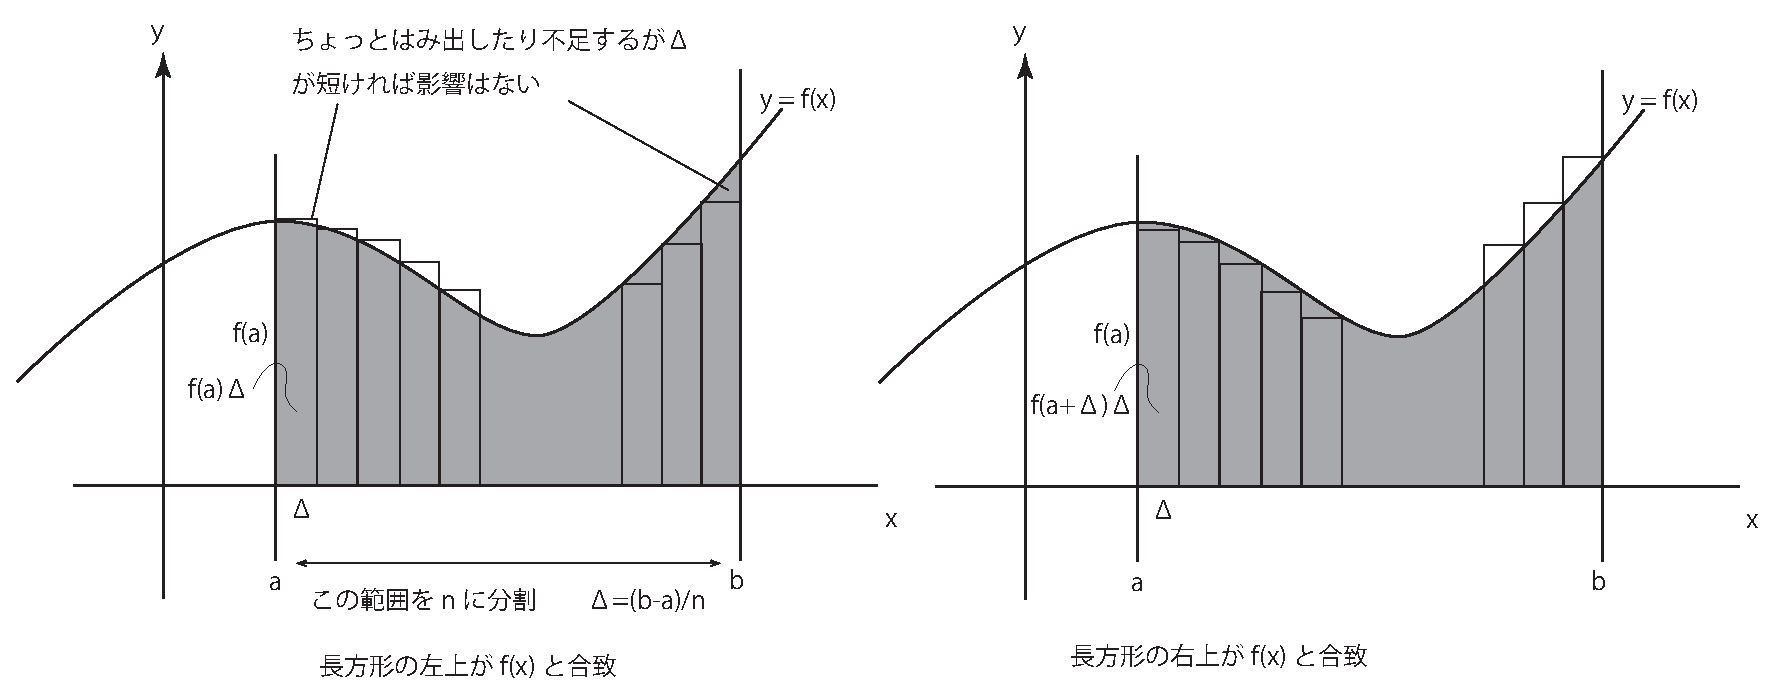
\includegraphics[width=9cm]{calculus12/surface2.eps}
\end{figure}
\end{itemize}
\end{slide}
\begin{slide}{区分求積法２}
\begin{itemize}
\item $n$区間に分割して$x_j = a + j\frac{b-a}{n} = a+j\Delta$とすれば長方形の面積の総和は
\begin{equation}
f(a)\Delta + f(a+\Delta)\Delta + \cdots + f(b-\Delta)\Delta = \sum_{j=0}^{n-1} f(x_j)\Delta  \nonumber
\end{equation}
\item 長方形の右上が$f(x)$と合致するようにする場合も同様に
%\begin{figure}[h]
%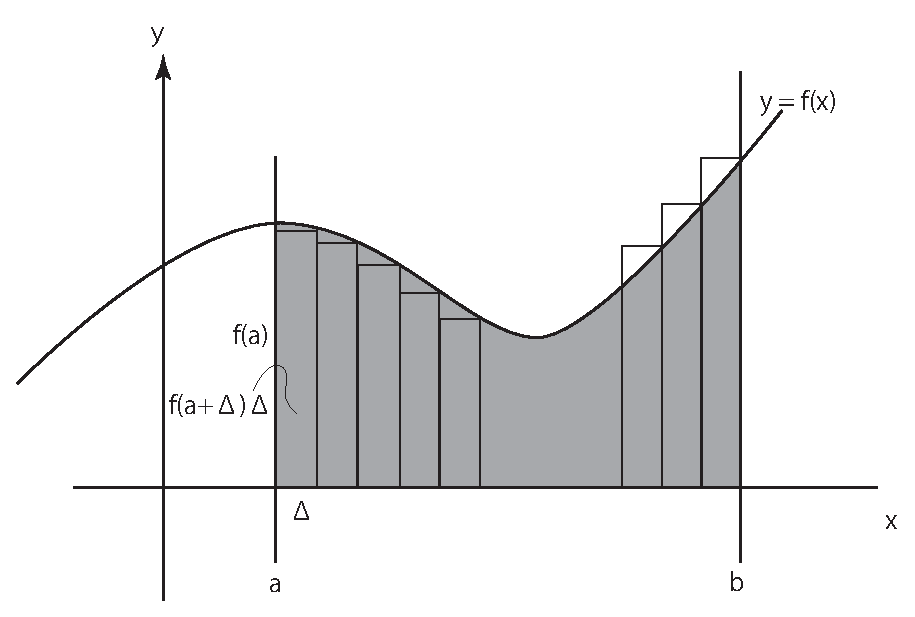
\includegraphics[width=4cm]{calculus12/surface3.eps}
%\end{figure}
\begin{equation}
f(a+\Delta)\Delta + f(a+\Delta)\Delta + \cdots + f(b)\Delta = \sum_{j=1}^{n} f(x_j)\Delta \nonumber
\end{equation}
どちらの場合も
\begin{equation}
\lim_{n\to \infty} \sum_{j=1}^n f(x_j) \Delta = \int_a^b f(x) dx \nonumber
\end{equation}
\end{itemize}
\end{slide}


%\begin{slide}{６．６　立体の体積}
%\begin{itemize}
%\item　下図の立体の$x=a$から$x=b$までの断面積を$S(x)$とすると、$x$から$x+dx$までの体積は
%\begin{figure}[h]
%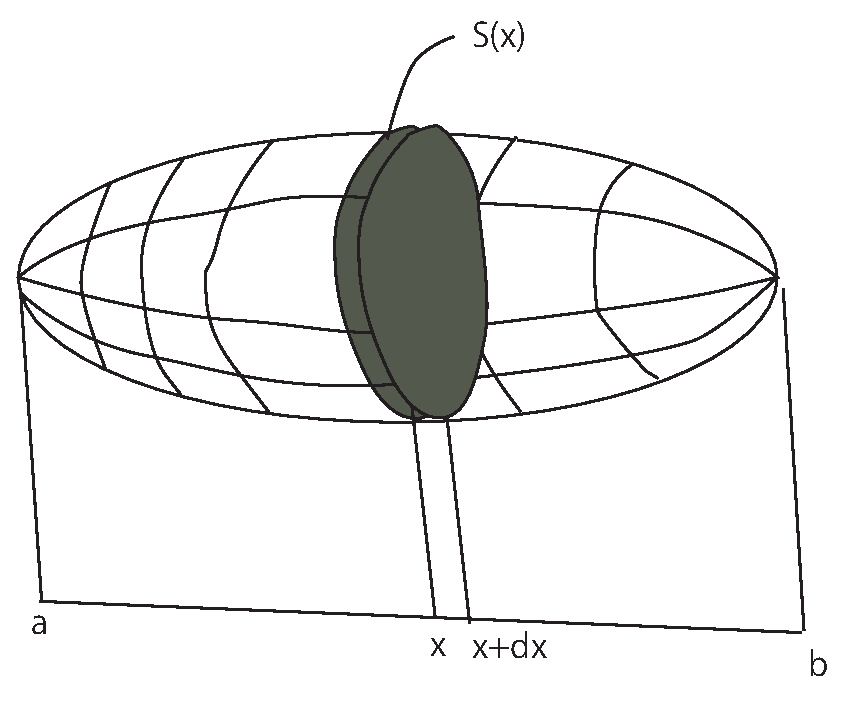
\includegraphics[width=4cm]{calculus12/vol.eps}
%\end{figure}
%\begin{equation}
%\Delta V = S(x)dx \nonumber
%\end{equation}
%したがって体積$V$は
%\begin{equation}
%V = \int_a^b S(x)dx \label{eq:vol}
%\end{equation}
%\end{itemize}
%\end{slide}
%\begin{slide}{定理６.１２}
%$y=g(x) \geqq 0$を$x$軸回りに回転して得られる立体の$a\leqq x \leqq b$の部分の体積$V$は
%\begin{equation}
%V = \pi \int_a^b g(x)^2 dx \nonumber
%\end{equation}
%\begin{figure}[h]
%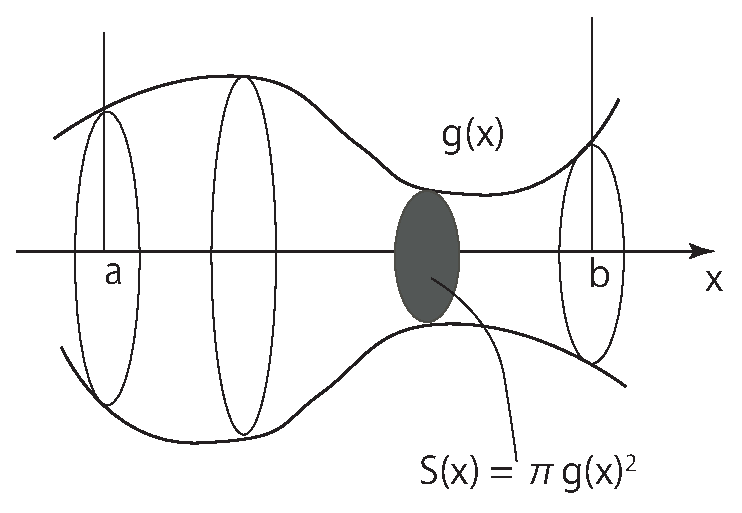
\includegraphics[width=5cm]{calculus12/rot.eps}
%
%$x$の位置での断面積は$S(x)=\pi g(x)^2$なので、式(\ref{eq:vol})を適用。
%\end{figure}
%\end{slide}
%\begin{slide}{例題６．８}
%\begin{itemize}
%\item $xy$平面の(0, 2)を中心とし半径1の円を$x$軸周りに回転してできる立体（トーラス:torus)の体積を求めよ。
%\begin{figure}[h]
%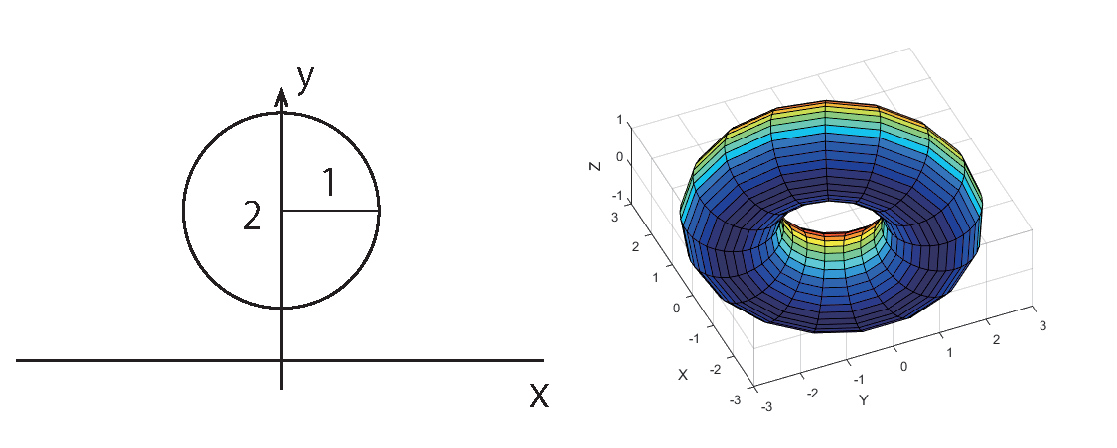
\includegraphics[width=5cm]{calculus12/torus.eps}
%\end{figure}
%\item 解答例
%円の上半分と下半分の方程式はそれぞれ以下となる。
%\begin{equation}
%y_u(x) =\sqrt{1-x^2} + 2, \qquad y_d(x) = -\sqrt{1-x^2}+2 \nonumber
%\end{equation}
%\begin{eqnarray}
%&& V = \pi \int_{-1}^{1} y_u^2 - y_d^2 dx \nonumber \\
%&=& \pi \int_{-1}^1 (\sqrt{1-x^2}+2)^2 - (-\sqrt{1-x^2}+2)^2dx \nonumber \\
%&=& 8\pi \int_{-1}^1 \sqrt{1-x^2} dx \label{eq:torus}
%\end{eqnarray}
%\end{itemize}
%\end{slide}
%\begin{slide}{例題６．８（２）}
%$x=\sin{\theta}$と置換すると、$\frac{dx}{d\theta}=\cos{\theta}$なので
%\begin{equation}
%\int_{-1}^1 \sqrt{1-x^2} dx = \int_{-\pi/2}^{\pi/2} \cos^2{\theta}d\theta \nonumber
%\end{equation}
%加法定理から$\cos^2{\theta} = \frac{1+\cos{2\theta}}{2}$なので
%\begin{equation}
%\int_{-1}^1 \sqrt{1-x^2} dx = \int_{-\pi/2}^{\pi/2} \frac{1}{2} d\theta= \frac{\pi}{2} \label{eq:double}
%\end{equation}
%式(\ref{eq:double})を式(\ref{eq:torus})に代入して
%\begin{equation}
%V = 4\pi^2 \nonumber 
%\end{equation}
%\end{slide}
%\begin{slide}{問題６．６}
%\begin{itemize}
%\item 定積分を用いて底面の半径$r$, 高さ$h$の直円錐(底面の円の中心と頂点とを結ぶ線が底面に垂直である円錐)の体積を求めよ
%\item 定積分を用いて半径$r$の球の体積を求めよ
%\end{itemize}
%\end{slide}
%\begin{slide}{６．７　曲線の長さ}
%\begin{itemize}
%\item $x,y$平面において、曲線$C$の上の点$(x,y)$が変数$t$の関数によって
%\begin{equation}
%x=f(t), \qquad y=g(t) \nonumber 
%\end{equation}
%の形に表されるとき、これを$C$のパラメータ表示といい、$t$をパラメタ（媒介変数: parameter)という。
%\item 例：原点$O$を中心とし半径$r$の円のパラメタ表示は
%
%\begin{equation}
%x = r\cos{\theta}, \qquad y=r\sin{\theta} \quad (0\leqq \theta \leqq 2\pi) \nonumber
%\end{equation}
%\end{itemize}
%\end{slide}
%\begin{slide}{曲線の長さ（２）}
%\begin{itemize}
%\item パラメタ$t$が$t+dt$に動く時の$x,y$は$f(t), g(t)$から$f(t+dt), g(t+dt)$に動くことになる。テイラー展開すると
%$f(t+dt) = f(t)+f'(x)dt$, $g(t+dt) = g(t)+ g'(t)dt$であり、曲線の伸び分は$\sqrt{f'(t)^2 + g'(t)^2}dt$となる。
%\begin{figure}[h]
%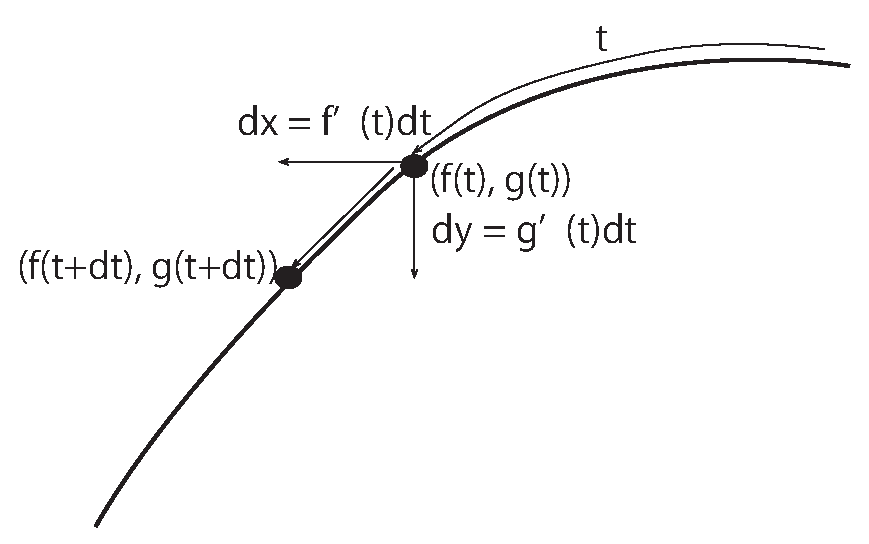
\includegraphics[width=5cm]{calculus12/curv.eps}
%\end{figure}
%\item $a \leqq t \leqq b$の長さ$l$は
%\begin{equation}
%l = \int_a^b \sqrt{f'(t)^2 + g'(t)^2} dt \nonumber
%\end{equation}
%\end{itemize}
%\end{slide}
%\begin{slide}{曲線の長さ：例}
%\begin{itemize}
%\item 原点$O$を中心とし半径$r$の円のパラメタ表示は
%\begin{equation}
%x = r\cos{\theta}, \qquad y=r\sin{\theta} \quad (0\leqq \theta \leqq 2\pi) \nonumber
%\end{equation}
%であり、$0 \leqq \theta \leqq \pi$の曲線の長さは
%\begin{eqnarray}
%&& \int_0^{\pi} \sqrt{r^2\sin^2{\theta} + r^2\cos^2{\theta}} d\theta \nonumber \\
%&=& \int_0^{\pi} r d\theta = \left[r\right]_0^{\pi} = \pi r \nonumber 
%\end{eqnarray}
%\end{itemize}
%\end{slide}
%
%\begin{slide}{曲線の長さ：補足}
%\begin{itemize}
%\item　$x,y$平面上の曲線がパラメタを用いずとも$y=g(x)$で求められる場合には $x=t$と考えて
%\begin{equation}
%f'(t) = 1 \qquad g'(t) = g'(x) = \frac{dy}{dx} \nonumber
%\end{equation}
%となるため以下となる。
%\begin{equation}
%l = \int_a^b \sqrt{1+\left(\frac{dy}{dx}\right)^2} dx \nonumber
%\end{equation}
%\end{itemize}
%\end{slide}
%\begin{slide}{例題６．１２}
%\begin{itemize}
%\item $y= \frac{e^x + e^{-x}}{2}$で与えられるとき、$-2 \leqq x \leqq 2$の曲線の長さを求めよ。
%\item 解答例: $\frac{dy}{dx} = \frac{e^x - e^{-x}}{2}$なので
%\begin{eqnarray}
%l &=& \int_{-2}^2 \sqrt{1+\frac{e^{2x} + e^{-2x} - 2}{4}} \nonumber \\
%&=& \int_{-2}^2 \sqrt{\frac{e^{2x} + e^{-2x}+2}{4}} = \int_{-2}^2 \frac{e^x + e^{-x}}{2} dx \nonumber \\
%&=& \frac{1}{2} \left[e^x - e^{-x}\right]_{-2}^2 = e^2 - e^{-2} \nonumber
%\end{eqnarray}
%\end{itemize}
%\end{slide}
%\begin{slide}{例題６．８ トーラス（３）}
%媒介変数$\theta$を導入
%\begin{figure}[h]
%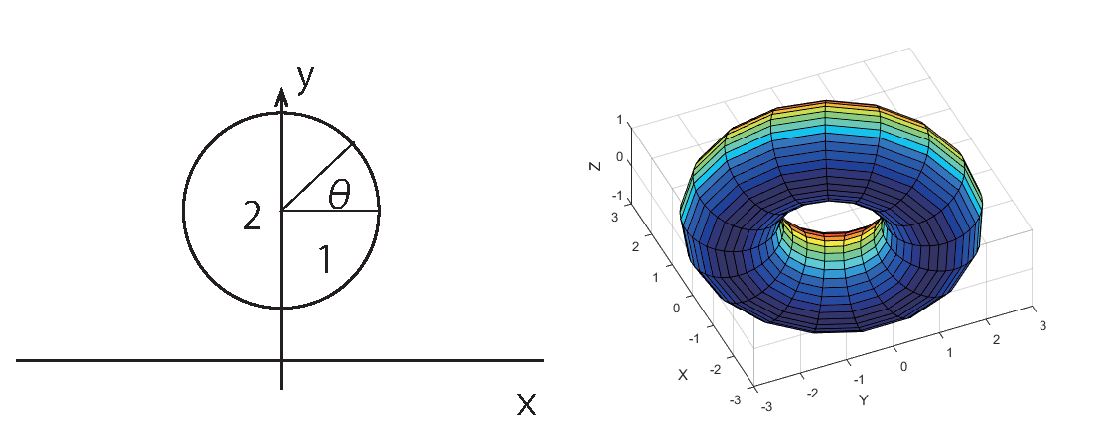
\includegraphics[width=5cm]{calculus12/torus2.eps}
%\end{figure}
%$\theta$と$x$の関係は
%\begin{equation}
%x=\cos\theta, \qquad \frac{dx}{d\theta} = -\sin\theta \nonumber 
%\end{equation}
%$\theta$の時のトーラスの断面積$S$は
%\begin{equation}
%S =\pi (2+\sin\theta)^2 - \pi(2-\sin\theta)^2 = 8\pi \sin\theta \nonumber
%\end{equation}
%なので体積$V= \int_{-1}^1 8\pi\sin\theta dx = -8\pi\int_{\pi}^{0} \sin^2\theta d\theta = 8\pi\int_{0}^{\pi} \sin^2\theta d\theta$ 、加法定理を利用して
%\begin{equation}
%V = 8\pi \int_{0}^{\pi} \frac{1-\cos{2\theta}}{2} dx =4\pi^2 \nonumber
%\end{equation}
%\end{slide}
%
